\documentclass[12pt, a4]{article}
\usepackage[english]{babel}
\usepackage[utf8x]{inputenc}
\usepackage{fullpage}
\usepackage{listings}
\usepackage{graphicx}
\usepackage{color}

%Syntax highlighting
\definecolor{blue-violet}{rgb}{0.54, 0.17, 0.89}
\definecolor{ao}{rgb}{0.0, 0.5, 0.0}
\definecolor{amaranth}{rgb}{0.9, 0.17, 0.31}
\definecolor{ballblue}{rgb}{0.13, 0.67, 0.8}
\definecolor{onyx}{rgb}{0.06, 0.06, 0.06}


\lstset{
  breaklines=true,                 % automatic line breaking only at whitespace
  captionpos=b,                    % sets the caption-position to bottom
  breakatwhitespace=false,
  keepspaces=true,
  numbers=left,
  numbersep=5pt,
  showspaces=false,
  showstringspaces=false,
  showtabs=false,
  tabsize=4,  
  backgroundcolor=\color{white},   % choose the background color
  commentstyle=\color{ao},    % comment style
  keywordstyle=\color{amaranth},    % keyword style
  stringstyle=\color{blue-violet},    % string literal style
  numberstyle=\tiny\color{ballblue},	   % number style
  basicstyle=\ttfamily\footnotesize\color{onyx} % size of fonts used for the code
}

%Document Header
\title{\textbf{Department of CSE\\SSN College of Engineering}}
\author{\textbf{Vishakan Subramanian - 18 5001 196 - Semester VII}}
\date{29 September 2021}

\begin{document}
\maketitle
\hrule
\section*{\center{UCS 1712 - Graphics And Multimedia Lab}}
\hrule
\bigskip

%Assignment Details
\subsection*{\center{\textbf{Exercise 7: Cohen-Sutherland Line Clipping in C++ Using OpenGL}}}
\subsection*{\flushleft{Aim:}}
\begin{flushleft}

Apply Cohen-Sutherland line clipping on a line $(x_1, y_1) (x_2, y_2)$ with respect to a clipping window $(X_Wmin, Y_Wmin) (X_Wmax, Y_Wmax)$. 

\bigskip
After clipping with respect to an edge, display the line segment with the calculated intermediate intersection points and the vertex list.\\

\bigskip
\textbf{Input:} The clipping window co-ordinates and the line endpoints.\\

\bigskip
\textbf{Note:} The output should show the clipping window and the line to be clipped in different colors.\\

\bigskip
You can show the intermediate steps using time delay. 
 
\end{flushleft}

%Code
\newpage
\subsection*{\flushleft{Code: Cohen-Sutherland Algorithm:}}
\begin{flushleft}
\lstinputlisting[language = C++]{CohenSutherland.cpp}
\end{flushleft}


%Output
\newpage
\subsection*{\flushleft{Output: Default Line \& Clipping Window}}
\begin{figure}[h]
\centering
\caption{Default Line \& Clipping Window}
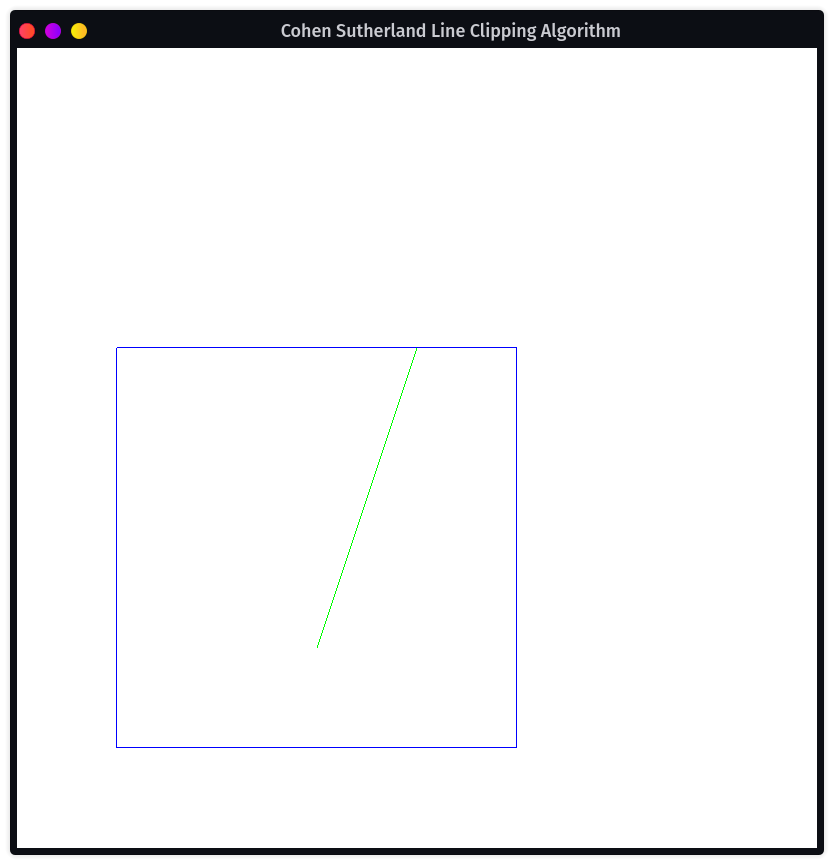
\includegraphics[height=15cm, width=15cm]{Outputs/Output-1.png}
\end{figure}

%Output
\newpage
\subsection*{\flushleft{Output: Console, Window[(100, 100), (500, 500)]}}
\begin{figure}[h]
\centering
\caption{Output: Console, Window[(100, 100), (500, 500)]}
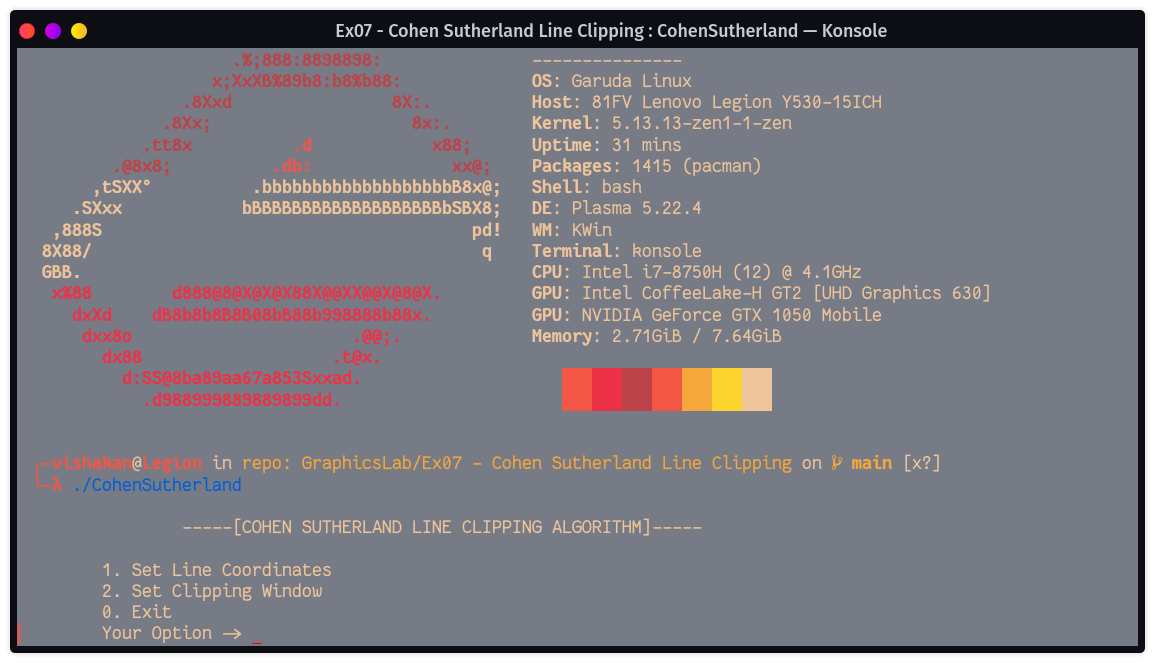
\includegraphics[height=12cm, width=17cm]{Outputs/Console-1.png}
\end{figure}

%Output
\newpage
\subsection*{\flushleft{Output: Window[(100, 100), (600, 600)]}}
\begin{figure}[h]
\centering
\caption{Output: Window[(100, 100), (600, 600)].}
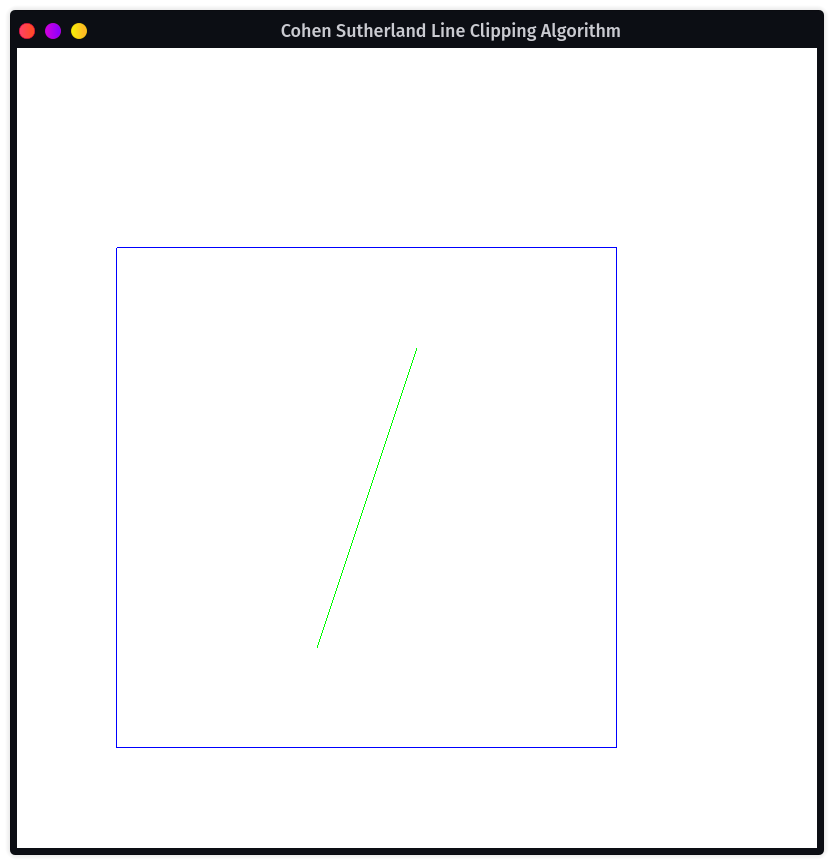
\includegraphics[height=15cm, width=15cm]{Outputs/Output-2.png}
\end{figure}

%Output
\newpage
\subsection*{\flushleft{Output: Console, Window[(100, 100), (600, 600)]}}
\begin{figure}[h]
\centering
\caption{Output: Console, Window[(100, 100), (600, 600)].}
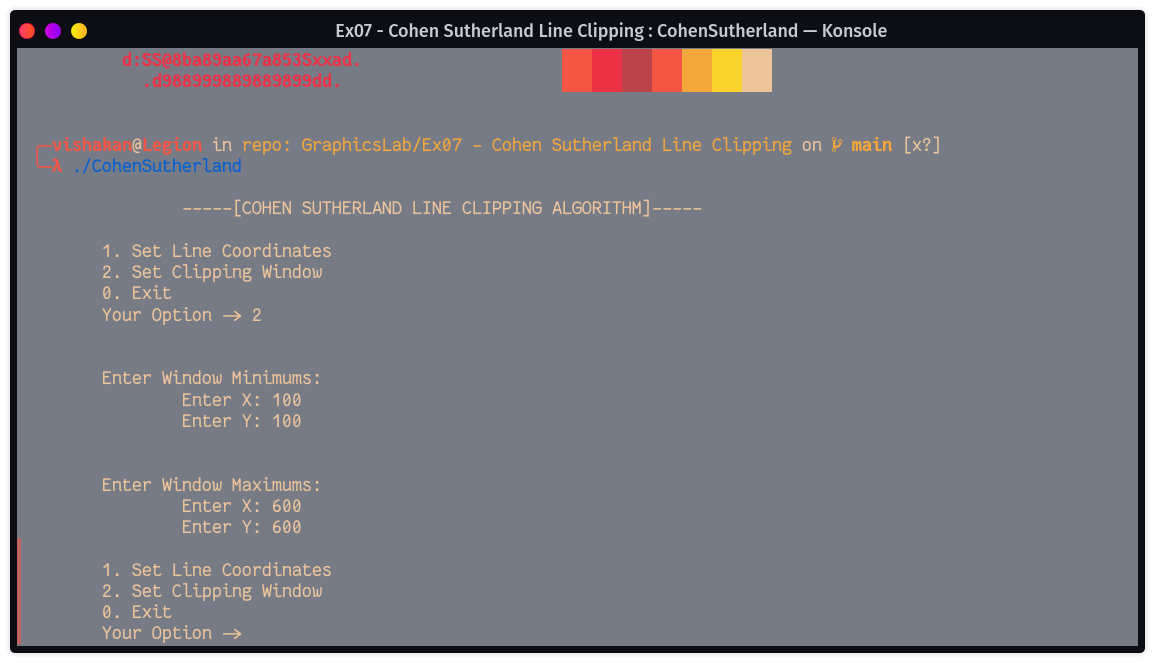
\includegraphics[height=12cm, width=17cm]{Outputs/Console-2.png}
\end{figure}

%Output
\newpage
\subsection*{\flushleft{Output: Line[(0, 0), (800, 800)] \& Clipping}}
\begin{figure}[h]
\centering
\caption{Output: Line[(0, 0), (800, 800)] \& Clipping.}
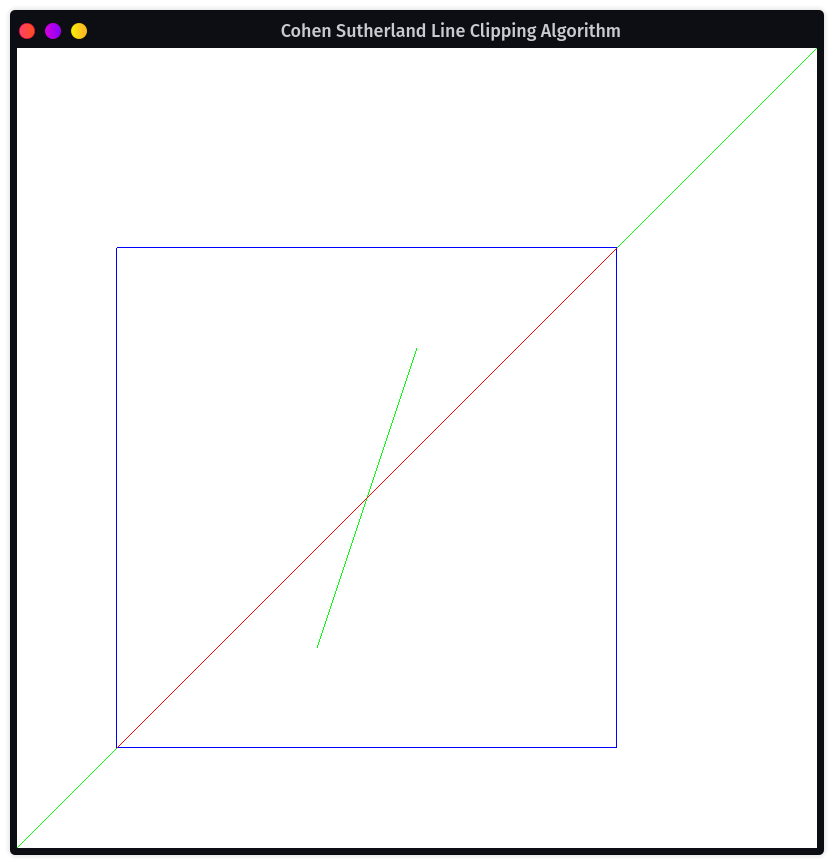
\includegraphics[height=15cm, width=15cm]{Outputs/Output-3.png}
\end{figure}

%Output
\newpage
\subsection*{\flushleft{Output: Console, Line[(0, 0), (800, 800)] \& Clipping}}
\begin{figure}[h]
\centering
\caption{Output: Console, Line[(0, 0), (800, 800)] \& Clipping.}
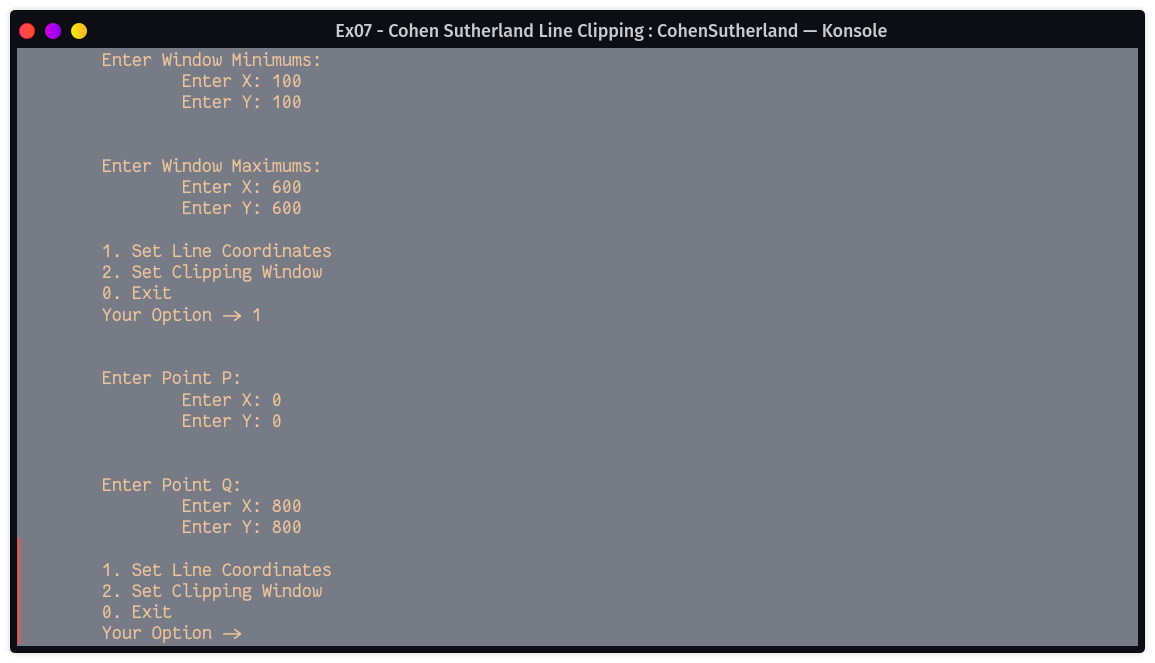
\includegraphics[height=12cm, width=17cm]{Outputs/Console-3.png}
\end{figure}

%Output
\newpage
\subsection*{\flushleft{Output: Line[(0, 700), (600, 700)] \& Clipping}}
\begin{figure}[h]
\centering
\caption{Output: Line[(0, 700), (600, 700)] \& Clipping.}
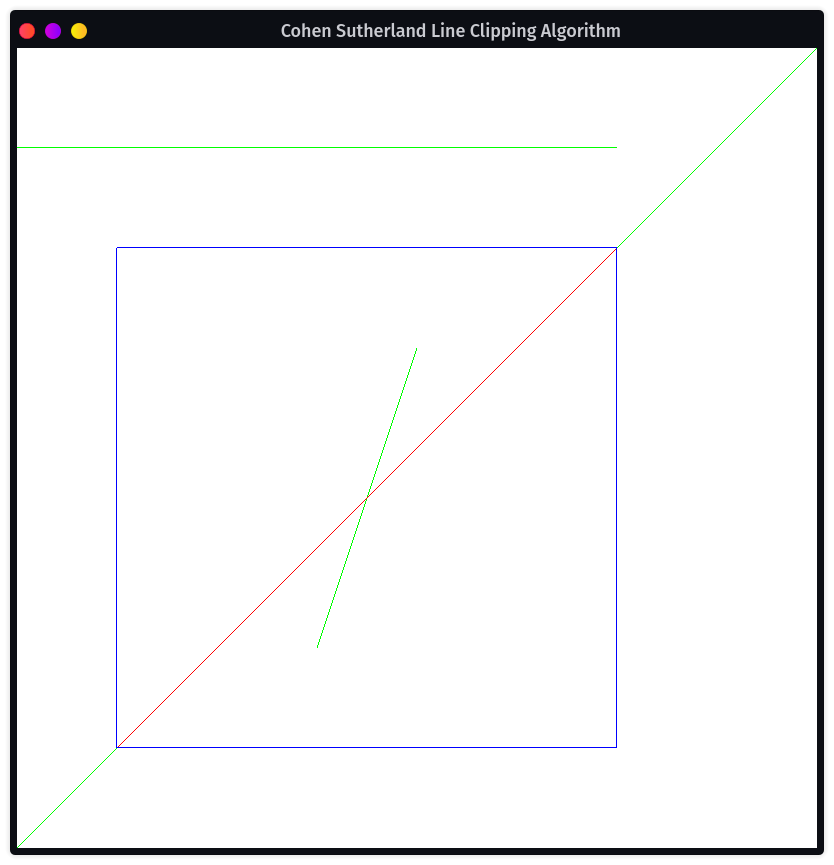
\includegraphics[height=15cm, width=15cm]{Outputs/Output-4.png}
\end{figure}

%Output
\newpage
\subsection*{\flushleft{Output: Console, Line[(0, 700), (600, 700)] \& Clipping}}
\begin{figure}[h]
\centering
\caption{Output: Console, Line[(0, 700), (600, 700)] \& Clipping.}
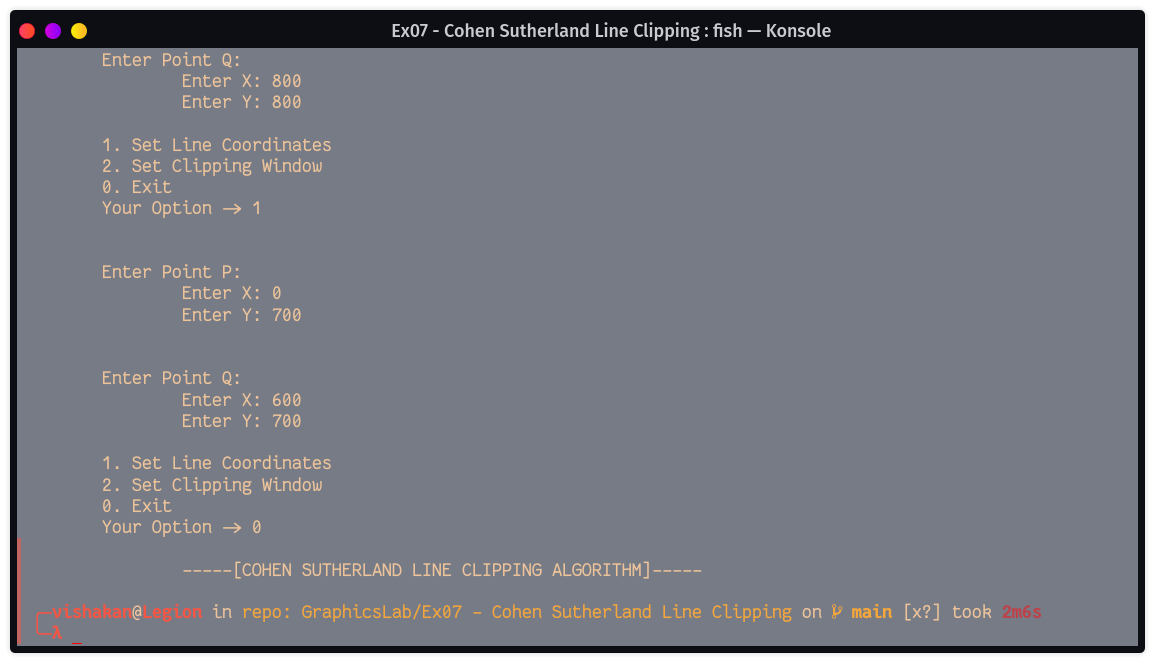
\includegraphics[height=12cm, width=17cm]{Outputs/Console-4.png}
\end{figure}


%Learning Outcome
\newpage
\subsection*{\flushleft{Learning Outcome:}}
\begin{itemize}
\item I learnt about \textbf{Cohen-Sutherland Line Clipping Algorithm}'s theoretical basis.
\item I learnt how to compute and program \textbf{Region Codes} for a given point and clipping window.
\item I understood about the advantages and pitfalls of the Cohen-Sutherland Algorithm.
\item I understood how to implement \textbf{trivial accept \& reject} conditions in the algorithm.
\item I was able to implement the algorithm for any given line and a rectangular clipping window region.
\item I demonstrated the clipped line, the original line and the clipping window using different colors.
\item I handled corner cases where $dx = 0$ and thus avoiding divide by zero errors in slope calculation.
\item I understood how to swap the points and continue clipping till region codes of both points become 0 for trivial acceptance.
\end{itemize}


\end{document}